\documentclass[a4paper]{article}
\usepackage{tabularx}
\usepackage[table]{xcolor}
\usepackage{graphicx}
\usepackage{datetime}
\usepackage{libertine}

\usepackage[xetex,%
            colorlinks=true,linkcolor=blue,citecolor=blue,%
            anchorcolor=red,urlcolor=blue,bookmarks=true,%
            bookmarksopen=true,bookmarksopenlevel=0,plainpages=false,%
            bookmarksnumbered=true,hyperindex=false,pdfstartview=,%
            pdfauthor={StuStaPay},%
            pdftitle={StuStaPay Bon},%
            %pdfsubject={StuStaPay Beleg}%
]{hyperref}


% for deterministic build
\special{pdf:trailerid [
    <00112233445566778899aabbccddeeff>
    <00112233445566778899aabbccddeeff>
]}

\begin{document}

    % reduce white space at beginning
    \title{\vspace{-6cm}}
    \date{}
    \maketitle
    % do not print a page number
    \thispagestyle{empty}


    \begin{center}
        \huge \VAR[config.title|latex]
    \end{center}

    % Rechnungsnummer und Datum
    \vspace{1cm}
    \textit{TEST \today - \currenttime } % for testing, to see if a new bon was created

    \textbf{Rechnung Nr. \VAR["{:010}".format(order.id)]} \hspace{\fill}  \VAR[order.booked_at.date()]

    % Addresse und Steuer ID
    \begin{flushright}
        \VAR[config.issuer|latex] \\
        \VAR[config.address.strip()|latex] \\
        USt-IdNr. \VAR[config.ust_id|latex] \\
    \end{flushright}

    % Line Items in the Rechnung
    \vspace{1cm}
    \newcolumntype{R}{>{\raggedleft\arraybackslash}X}
    \rowcolors{2}{}{gray!40}
    \begin{tabularx}{\textwidth}{ p{1cm} p{4cm} R R X }
        ~                    & \textbf{Produkt}        & \textbf{Einzelpreis}   & \textbf{Gesamt}              &                       \\
        \hline
        \BLOCK[ for item in order.line_items ]
        \VAR[item.quantity]x & \VAR[item.product.name] & \VAR[item.product_price|money] & \VAR[item.total_price|money] & [\VAR[item.tax_name]] \\
        \BLOCK[endfor]
    \end{tabularx}


    % Gesamtsumme
    \vspace{1cm}
    \hspace{\fill} \textbf{Summe EUR} \textbf{\VAR[order.total_price|money]€}

    %Steuerstatz
    \vspace{1cm}
    \rowcolors{0}{}{}
    \begin{tabularx}{\textwidth}{ RRRR }
        \textbf{MwSt.\%}                                         & \textbf{Brutto}                & \textbf{Netto}                   & \textbf{MwSt.}                 \\
        \hline
        \BLOCK[for tax_rate in tax_rate_aggregations ]
        \VAR[tax_rate.tax_name]=\VAR[tax_rate.tax_rate|percent] & \VAR[tax_rate.total_price|money] & \VAR[tax_rate.total_no_tax|money] & \VAR[tax_rate.total_tax|money] \\
        \BLOCK[endfor]
        \hline
        ~                                                        & \VAR[order.total_price|money]    & \VAR[order.total_no_tax|money]    & \VAR[order.total_tax|money]    \\
    \end{tabularx}

    % sonstige Infos
    \vspace{1cm}
    \begin{tabularx}{\textwidth}{ Rp{3cm} }
        Zahlmethode:        & \VAR[order.payment_method.name]    \\
% We use the TSE start and stop time instead of our order booking time
%         Vorgangszeitpunkt:  & \VAR[order.booked_at.astimezone()]  \\
        Kassierer:          & \VAR[order.cashier_id]  \\
        Seriennummer Kasse: & \VAR[order.till_id]     \\
        \BLOCK[if order.signature_status == "done"]
        Transaktionsnummer: & \VAR[order.tse_transaction|latex] \\
        Signaturzähler:     & \VAR[order.tse_signaturenr|latex] \\
        Signatur:           & \VAR[order.tse_signature|latex] \\
        Start-Zeit:         & \VAR[order.tse_start|latex] \\
        Stop-Zeit:          & \VAR[order.tse_end|latex] \\
        Public-Key          & \VAR[order.tse_public_key|latex] \\
        Hash-Algorithmus:   & \VAR[order.tse_hashalgo|latex] \\
        Zeitformat:         & \VAR[order.tse_time_format|latex] \\
        QR-Code             & \VAR[order.tse_qr_code_text|latex] \\
        \BLOCK[else]
        TSE                 & ausgefallen \\
        \BLOCK[endif]
    \end{tabularx}

    % evtl direkter online Link um die Rechnung abzurufen

    % ein kurzer "witz"
    \vspace{\fill}
    \begin{center}
        \VAR[closing_text|latex]

        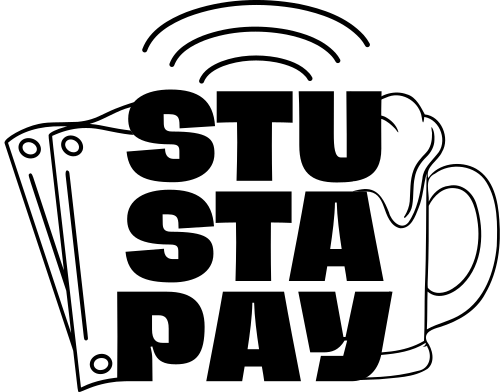
\includegraphics[width=3cm]{logo}
    \end{center}

\end{document}
